\documentclass[8pt]{beamer}
\usetheme{Montpellier} 
\usepackage{lmodern}
\usepackage{amsmath}
\usepackage[utf8]{inputenc}
\usepackage[T1]{fontenc}
\usepackage{polski}
\usepackage[polish]{babel}


\newcommand{\argmax}[1]{\underset{#1}{\operatorname{arg}\,\operatorname{max}}\;}
\beamertemplatenavigationsymbolsempty

\makeatletter
\setbeamertemplate{footline}
{
  \leavevmode%
  \hbox{%
  \begin{beamercolorbox}[wd=.333333\paperwidth,ht=2.25ex,dp=1ex,center]{author in head/foot}%
    \usebeamerfont{author in head/foot}\insertshortauthor~~\beamer@ifempty{\insertshortinstitute}{}{(\insertshortinstitute)}
  \end{beamercolorbox}%
  \begin{beamercolorbox}[wd=.333333\paperwidth,ht=2.25ex,dp=1ex,center]{title in head/foot}%
    \usebeamerfont{title in head/foot}\insertshorttitle
  \end{beamercolorbox}%
  \begin{beamercolorbox}[wd=.333333\paperwidth,ht=2.25ex,dp=1ex,right]{date in head/foot}%
    \usebeamerfont{date in head/foot}\insertshortdate{}\hspace*{2em}
    \insertframenumber\hspace*{2ex} 
  \end{beamercolorbox}}%
  \vskip0pt%
}
\makeatother


\author[Adam Kosiorek]{Adam Kosiorek\\ \footnotesize pod kierunkiem prof. dr hab. B. Siemiątkowskiej}
\begin{document}
\title[Rozpoznawanie obiektów 3D na podstawie danych RGBD]{\HUGE Politechnika Warszawska\\ Wydział Mechatroniki \\ \ \\ \Large Rozpoznawanie obiektów 3D na podstawie danych RGBD} 
\date{11 lutego 2014} 

\thispagestyle{empty}
\titlepage
\thispagestyle{empty}
\frame{\frametitle{Spis treści}\tableofcontents}
\begin{document}

\section{Założenia i zakres pracy} 

\begin{frame}{Założenia}
  %\setcounter{framenumber}{1}
   
   Założeniem pracy jest zbadanie zagadnienia klasyfikacji metodą Bag of Words obiektów 3D na podstawie zdjęć RGBD. Zdjęcia powinny byc reprezentowane w formie chmur punktów. Ponadto zakłada się, że: \ \\
  \begin{itemize}
   \item Analizowane dane pochodzą z kamery RGBD Microsoft Kinect
   \item Implementacja algorytmu w języku C++ z wykorzystaniem bibliotek OpenCV i/lub PointCloud Library
   \item Testy aplikacji na ogólnie dostępnej, naukowej bazie danych
  \end{itemize}

\end{frame}

\begin{frame}{Zakres pracy}
  \begin{enumerate}
    \item Przegląd istniejących rozwiązań dotyczących klasyfikacji obiektów na podstawie chmur punktów
    \item Opracowanie algorytmu klasyfikacji obiektów na podstawie chmur punktów
    \item Implementacja algorytmu w języku C++ 
    \item Przeprowadzenie testów szybkości oraz skuteczności klasyfikacji 
    \item Opracowanie wniosków końcowych
  \end{enumerate}
\end{frame}


\section{Podejście Bag of Words}
\begin{frame} {Bag of Words - Wprowadzenie}
  \begin{figure}
    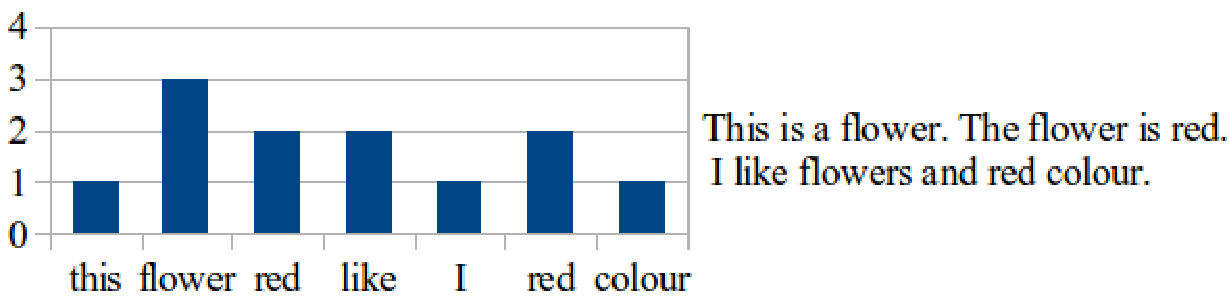
\includegraphics[scale=0.3]{../figs/bow_example-eps-converted-to}
  \end{figure}
  
  \begin{itemize}
   \item Częstośc występowania słów
   \item Usunięcie gramatyki, kolejności słów
   \item Histogram jako forma pośrednia
   \item Wymaga utworzenia słownika
   \item Reprezentacja rzadka w przypadku dużego słownika
   \item Używany m. in. do znajdowania rozkładu tematów w obrazie
  \end{itemize}


\end{frame}

\begin{frame}{Bag of Words w obrazach}	
	\begin{columns}
	
	 \begin{column}{6cm}
	 \begin{figure}
	   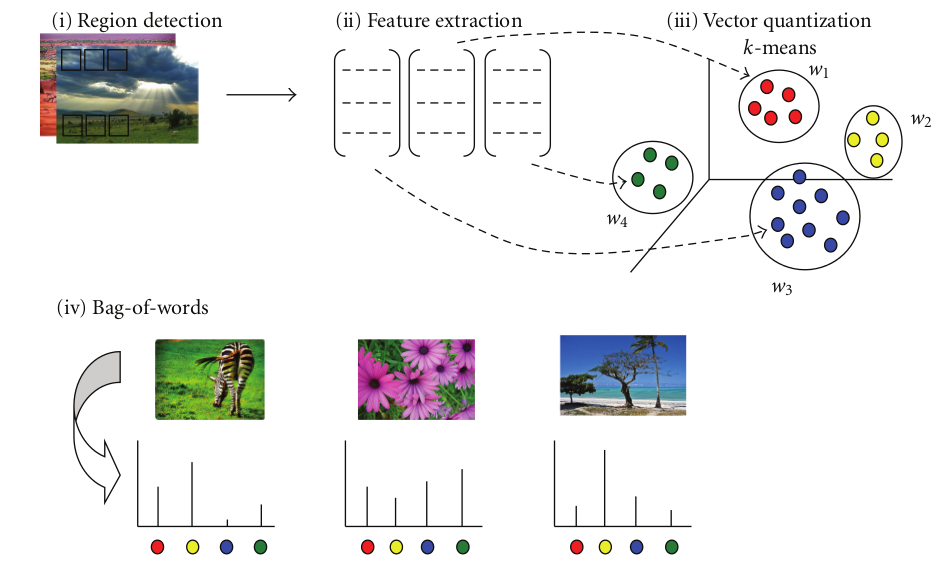
\includegraphics[scale=0.15]{../figs/tsai2012}
	   \end{figure}
	 \end{column}
	 
	 \begin{column}{3cm}
	  \footnotesize Grafika pochodzi z C. Tsai. \textit{Bag-of-words representation in image annotation: A review. ISN Artificial Intelligence, 2012}.
	 \end{column}

	\end{columns}

	\begin{enumerate}
	 \item Wykrycie punktów charakterystycznych
	 \begin{itemize}
	  \item współrzędne (x, y) oraz skala obrazka
	 \end{itemize}

	 \item Opisanie otoczenia wykrytych punktów
	 \begin{itemize}
 	  \item opis jednoznaczny, zazwyczaj poprzez przestrzenny histogram gradientów
	 \end{itemize}
	 \item Budowanie słownika i kwantyzacja
	 \begin{itemize}
	  \item punkty układają się w obszary, które można wykryć - klasteryzacja
	 \end{itemize}
	 \item Klasyfikacja
	 \begin{itemize}
	  \item klasyfikator uczący się - Support Vector Machine, Modele graficzne, Boosting
	 \end{itemize}
	\end{enumerate}	
\end{frame}{}

\section{Projekt Aplikacji}

\begin{frame}{Projekt Aplikacji}
	 \begin{columns}
	
	 \begin{column}{6cm}
	  \begin{figure}
	    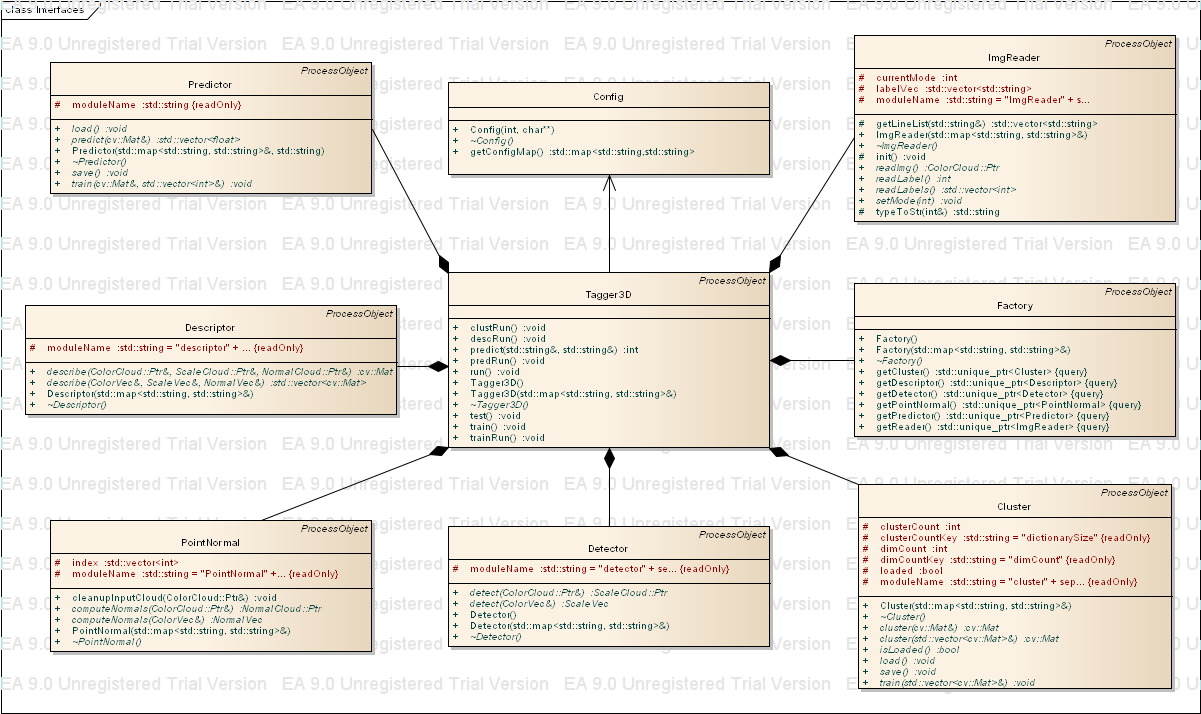
\includegraphics[width=1.0\textwidth]{../figs/class}	   
	  \end{figure}
	  \centering \footnotesize Architektura
	 \end{column}
	 
	 \begin{column}{6cm}
	  \begin{figure}
	  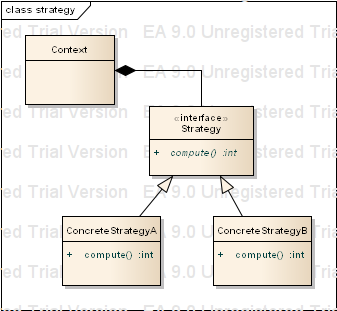
\includegraphics[width=0.5\textwidth]{../figs/strategy}	
	  \end{figure}
	  \centering \footnotesize Strategia
	 \end{column}
	 
	\end{columns}
	
  \begin{columns}

    \begin{column}{6cm}
    \begin{itemize}
    \item Główny obiekt \textit{Tagger3D} zarządza całą aplikacją
    \item Fabryka odpowiedzialna za tworzenie innych obiektów, konfigurowana w czasie działania programu
    \item Każdy etap procesu BoW ma wydzielony interfejs - wzorzec projektowy Strategia
      \begin{itemize}
	\item Detector, Descriptor itd.
      \end{itemize}
    \end{itemize}

    \end{column}

    \begin{column}{6cm}
    \begin{itemize}
     \item Strategia umożliwia wymianę algorytmów w czasie działania programu, w sposób niewidzialny dla aplikacji
     \item Konfiguracja w pliku tekstowym
     \item Obiekt IoUtils oparty o szablony obsługuje operacje wejścia/wyjścia
    \end{itemize}

    \end{column}

    \end{columns}
\end{frame}

\section{Bazy danych}

\begin{frame}{Berkely 3D Object Dataset}

	\begin{columns}
	
	 \begin{column}{6cm}
	 \begin{figure}[!ht]
	    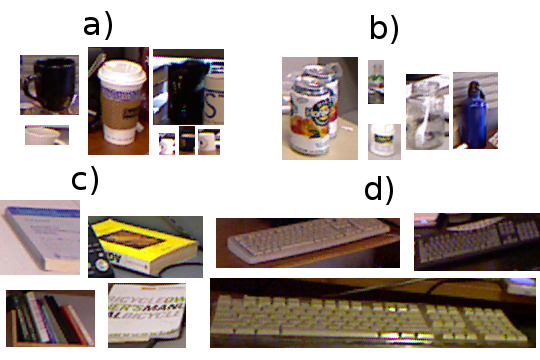
\includegraphics[width=0.65\textwidth]{../figs/b3do_objects}
	  \footnotesize \caption{Obiekty z B3DO. Zdjęcia w oryginalnej jakości. a) kubek b) butelka c) książka d) klawiatura}
	  \label{fig:b3do_objects}
	  \end{figure}
	 \end{column}
	 
	  \begin{column}{6cm}	  
	  \begin{itemize}
	   \item 78 kategorii obiektów
	   \item Wiele obiektów na jednym zdjęciu
	   \item Niska jakość zdjęć, wiele zdjęć niedoświetlonych, zaszumionych
	   \item Obiekty przysłonięte
	   \item Kolorowe zdjęcia i mapy głębi; Adnoacje w XML
	   \item Skrypty w Pythonie i C++ do ekstrakcji pojedynczych obiektów i podziału na kategorie.
	   \item Od 1 do 299 instancji w jednej kategorii
	   \item Losowy wybór 8 kategorii tak, żeby było~>~50 instancji w każdej kategorii
	  \end{itemize}

	  
	 \end{column}
	\end{columns}	
\end{frame}

\begin{frame}{University of Tokyo Dataset}
	\begin{figure}[!ht]
	\centering
	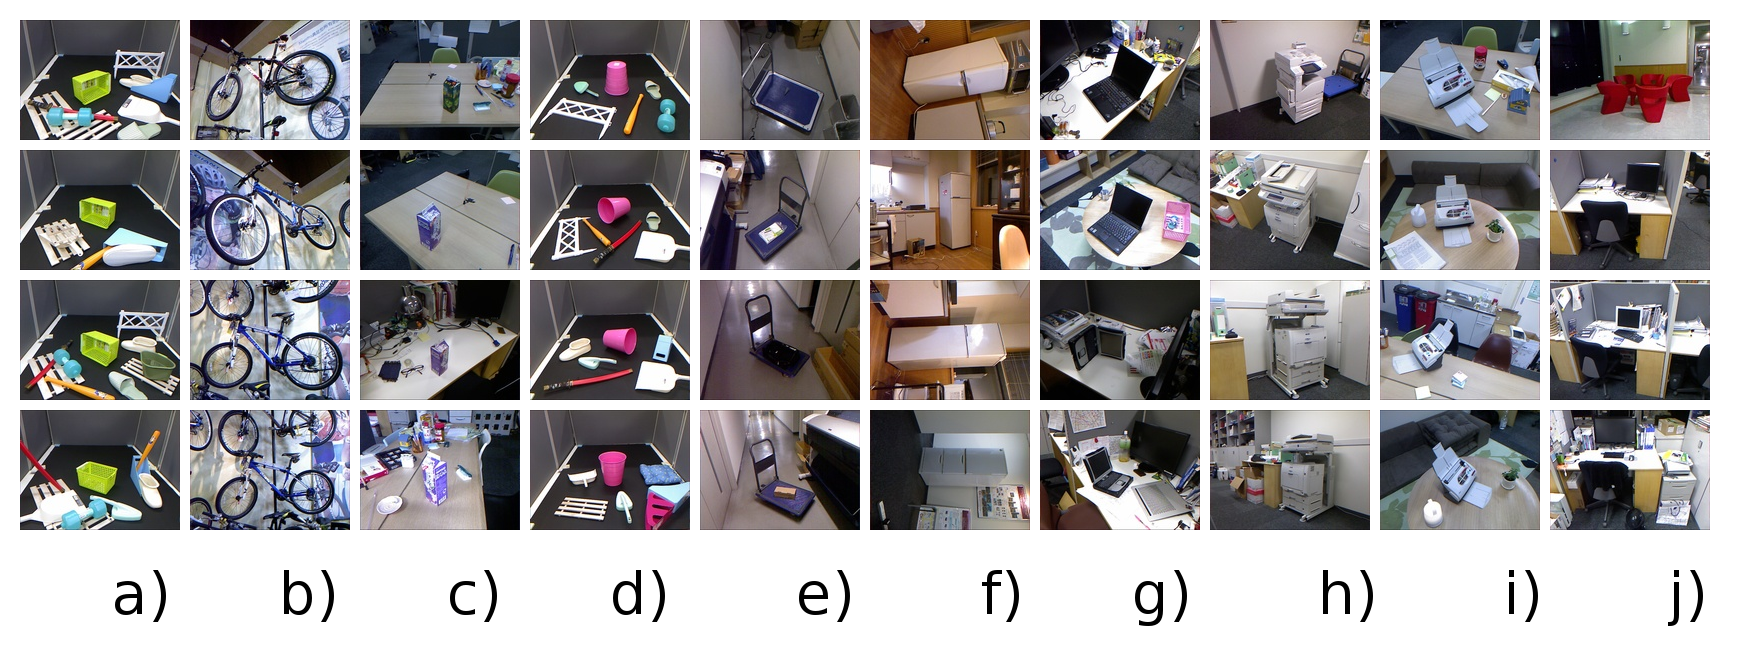
\includegraphics[width=0.6\textwidth]{../figs/tokyo_horizontal}
	\footnotesize \caption{The Tokyo dataset: a) kosz b) rower c) pudełko d) wiadro e) wózek f) lodówka g) notebook h) drukarka i) skaner j) scena}
	\label{fig:tokyo}
	\end{figure}
	
		\begin{columns}
		\begin{column}{6cm}
			\begin{itemize}
			\item 10 kategorii
			\item 1 obiekt (oznaczony) na zdjęciu	
			\item Mogą być obiekty nieoznaczone, których nie należy brać pod uwagę
			\item Zdjęcia dobrej jakości, dobrze naświetlone
			\item Wszystkie zdjęcia w kategorii to instancje jednego obiektu
			\end{itemize}
		\end{column}
		\begin{column}{7cm}     
			\begin{itemize}
			%\setcounter{enumi}{3}
			\item Skomplikowane sceny
			\item Małe różnice pomiędzy klasami obiektów
			  \begin{itemize}
			  \item skaner i drukarka
			  \item koszyk i wiadro
			  \end{itemize}
			  \item Dane w formie kolorowe: zdjęcie + plik .csv z absolutnymi współrzędnymi wszystkich pixeli
			  \item Skrypty Python i C++ - przeksztąłcenie do chmury punktów w formacie PCD
			\end{itemize}
		\end{column}
	\end{columns}

\end{frame}

\section{Wyniki i podsumowanie}

\begin{frame}{Porównanie algorytmów}

	\begin{columns}
	
	\begin{column}{5cm}
	\begin{table}[!ht]	
	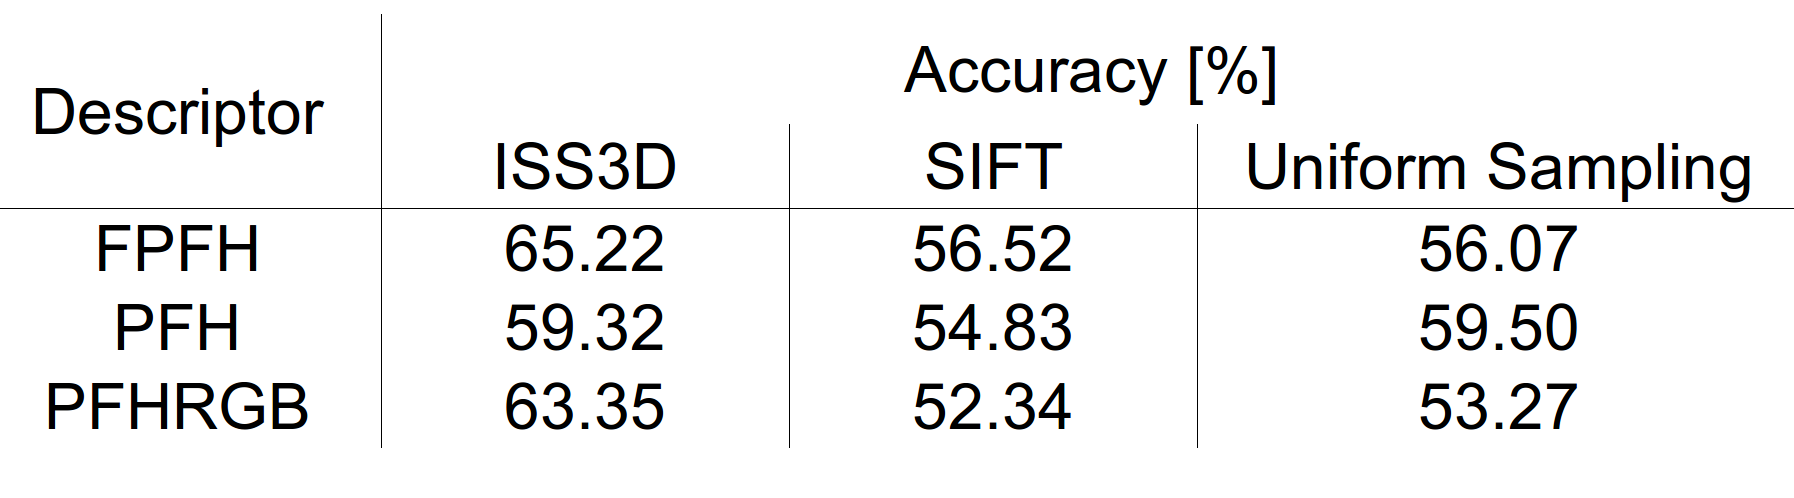
\includegraphics[scale=0.08]{../figs/desc_b3do} \\ 
	\centering
	\footnotesize Porównanie algorytmów. \\
	\vspace{1cm}
	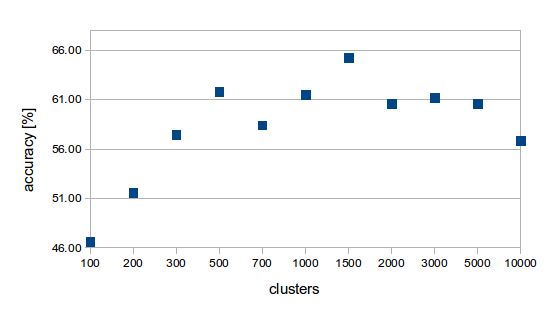
\includegraphics[scale=0.2]{../figs/clustering_centroids_b3do} \\ 
	\centering
	\footnotesize Wpływ rozmiaru słownika na skuteczność klasyfikacji.
	\end{table}
	
	 \end{column}
	 
	  \begin{column}{7cm}	  
	  \begin{itemize}
	   \item Wstępna selekcja algorytmów na podstawie przeglądu literatury
	   \item Rodzina deskryptorów PFH uzyskuje najlepsze wyniki w dopasowywaniu chmur punktów:
	    \begin{description}
	      \item[PFH] Algorytm bazowy, 125 wymiarów
	      \item[FPFH] Algorytm przybliżony, 33 wymiary
	      \item[PFHRGB] Algorytm uwzględnia kolor, 250 wymiarów
	    \end{description}
	   \item Detektory: 
	       \begin{description}
	      \item[SIFT] Najlepszy algorytm 2D
	      \item[ISS] Najlepsze wyniki w dopasowywaniu chmur punktów
	      \item[US] Najprostszy, równomierna siatka punktów
	    \end{description}
	   \item Optymalny rozmiar słownika
	  \end{itemize}

	  
	 \end{column}
	\end{columns}
	
\end{frame}

\begin{frame}{Wyniki B3DO}
		\begin{columns}
	
	 \begin{column}{6cm}
	\begin{table}[!ht]	
	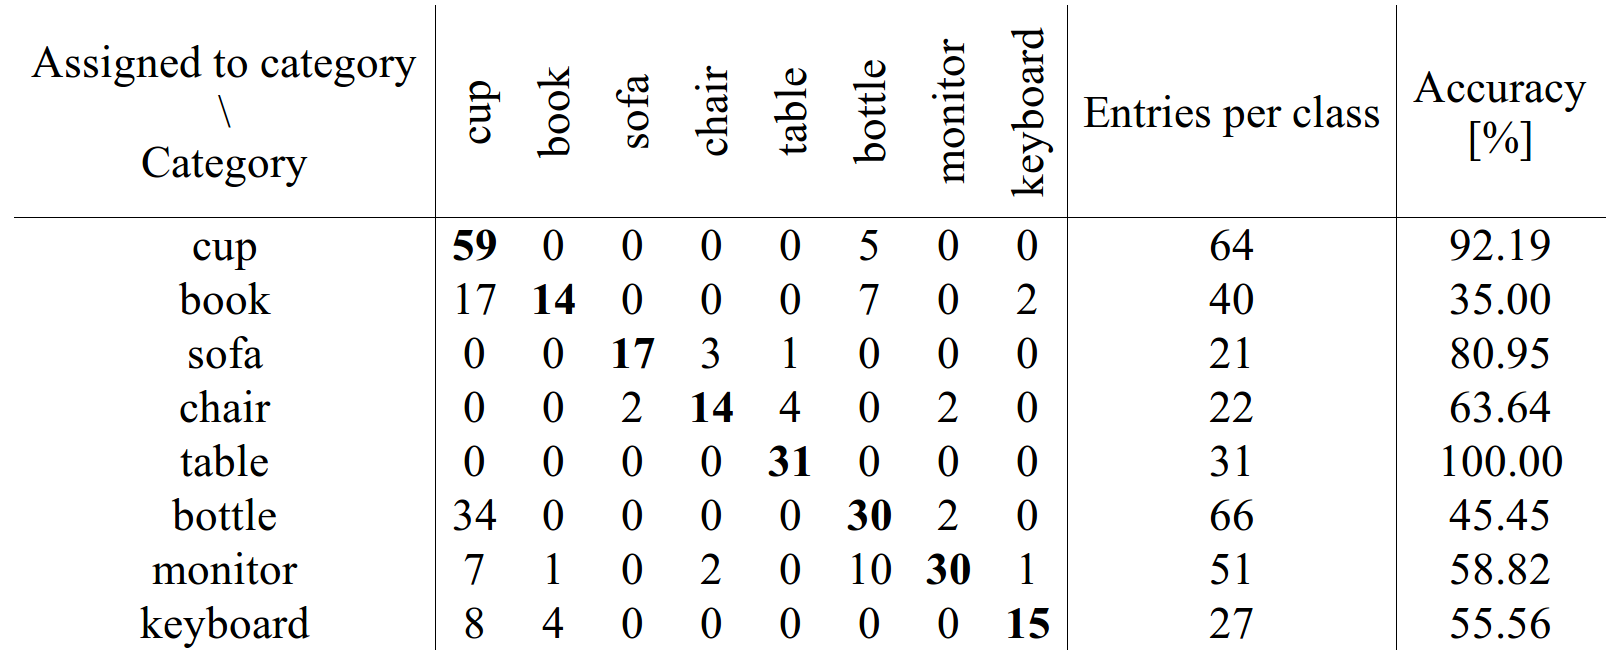
\includegraphics[scale=0.1]{../figs/b3do_conf_matrix}	\\ \ \\
	\centering
	\footnotesize \textbf{Wynik: 65.22\%} Wyniki na bazie B3DO, detektor ISS, ekstraktor FPFH, słownik o wielkości 1500 słów.
	\end{table}
	 \end{column}
	 
	  \begin{column}{6cm}	  
	  \begin{itemize}
	   \item Im lepiej rozdzielone kategorie obiektów, tym wyższa wyniki
	   \item Najwyższy wynik: stół, 100\%
	   \item Niskie wyniki wynikają bezpośrednio z podobieństwa między klasami: 
	   \begin{itemize}
	    \item książka, 35\%, mylona z filiżanką i butelką
	    \item butelka, 45\%, mylona z filiżanką
	   \end{itemize}
	  \end{itemize}
	  
	 \end{column}
	\end{columns}	
\end{frame}

\begin{frame}{Wyniki Tokyo}
	\begin{columns}
	
	 \begin{column}{5cm}
	\begin{table}[!ht]	
	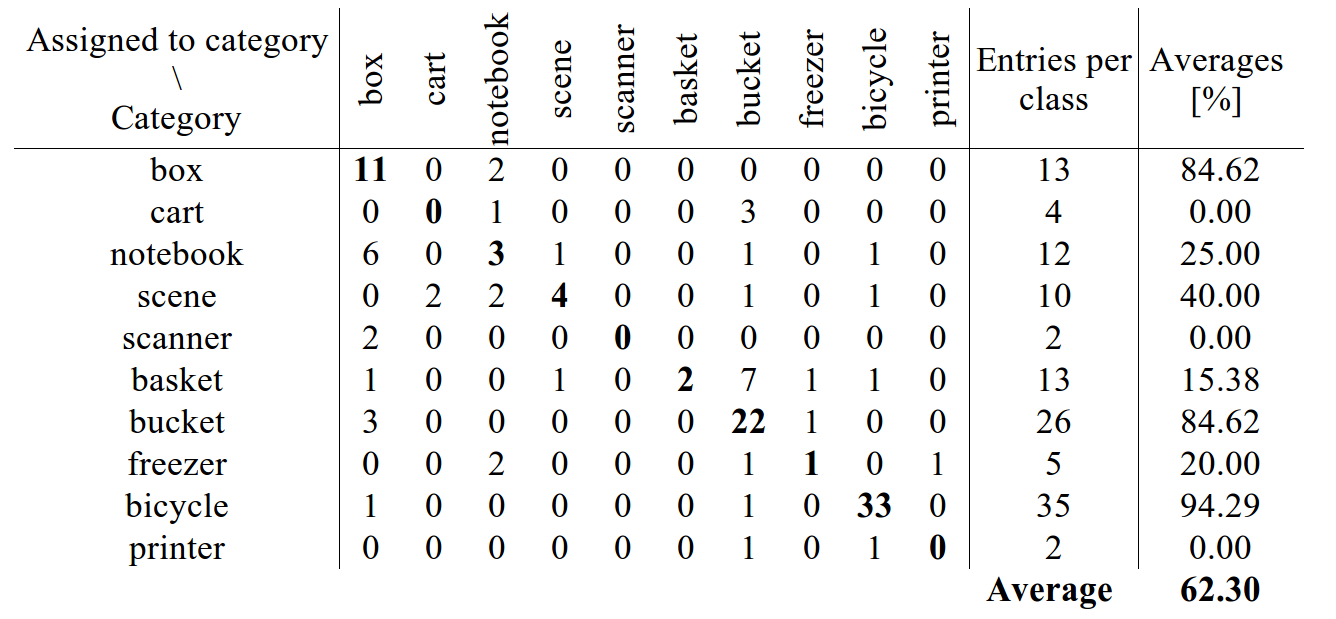
\includegraphics[scale=0.1]{../figs/tokyo_conf_matrix} \\ \ \\
	\centering
	\footnotesize \textbf{Wynik: 62.30\%} Wyniki na bazie Tokyo, detektor ISS, ekstraktor PFH, słownik o wielkości 3000 słów.
	\end{table}
	
	 \end{column}
	 
	  \begin{column}{6cm}	  
	  \begin{itemize}
	   \item Wyraźna zależność między ilością instancji w danej klasie i skutecznością klasyfikacji
	   \item Najwyższy wynik: rower, 94\%, największa ilośc obiektów
	   \item Najniższe wyniki przy klasach, w których są odpowiednio 4, 2 i 2 obiekty: 
	    \begin{itemize}
	      \item wózek, 0\%
	      \item skaner, 0\%
	      \item drukarka, 0\%
	    \end{itemize}
	   \item Notebook jest mylon z pudełkiem
	   \item Wiadro jest mylone z pudełkiem
	   \item Kosz jest mylony z wiadrem
	  \end{itemize}
	  
	 \end{column}
	\end{columns}	
\end{frame}

\begin{frame}{Podsumowanie}
	\begin{itemize}
	 \item Uzyskane wyniki na bazach B3DO i TOKYO są odpowiednio $5.21$ i $6.23$ razy lepsze od kategoryzacji losowej (odpowiednio 12.5\% i 10\%)
	 \item Zrealizowano wszystkie założenia projektowe
	 \item Wystąpiły następujące problemy
	  \begin{itemize}
	    \item W zasadzie brak baz danych nadających się do zadania klasyfikacji obiektów na podstawie danych RGBD
	    \item Bardzo wymagające przetwarzanie chmur punktów ze względu na brak jakiejkolwiek struktury
	    \item Najlepsze algorytmy dostępne są tylko do 2D, brak możliwości ich prostego uogólnienia do 3D
	  \end{itemize}
	  
	  \item Możliwości poprawy skuteczności i/lub szybkości działania aplikacji:
	    \begin{itemize}
	      \item Przeniesienie obliczeń do domeny 2D; RGB i D jako niezależne obrazy + złożenie wyników klasyfikacji
	      \item Trening klasyfikatorów na znacznie większych bazach danych
	      \item Przeniesienie obliczeń na GPU
	    \end{itemize}
	    
	\end{itemize}

\end{frame}

\end{document}

